\documentclass{mybeamer}
\usepackage[all,cmtip]{xy}
\usepackage{lipsum}
\title{Dinámica efectiva de un sistema de N qubits}
\subtitle{Utilizando el principio de máxima entropía}
\author[A. Castillo Guerrero]{Autor: A. Castillo\\ Director de tesis: D. Dávalos\\ Equipo de trabajo: C. Pineda, D. Dávalos, K. Uriostegui, E. Navarrete.}
\date{Enero 2023} % or whatever the date you are presenting in is
\institute[Facultad de Ciencias, UNAM]{Facultad de Ciencias, UNAM}
% \copyrightnotice{Published by the American Institute of Aeronautics and Astronautics, Inc., with permission}

\begin{document}

\maketitle

\cutoc
\section{Problem statement}

\begin{frame}{Blurry, low resolution measurement tool}
    \begin{itemize}
        \item Faulty instrumentation.
        \item Can only resolve one particle.
        \item May measure the wrong particle.
    \end{itemize}
    \begin{equation*}
        \mcC[\varrho]=\Tr_{2}[(1-p)\varrho+pS\varrho S^{\dag}].
    \end{equation*}
\end{frame}

\begin{frame}{Effective dynamics}
    \begin{columns}
        \begin{column}{0.5\textwidth}
            \begin{itemize}
                \item Microscopic evolution is known.
                \item \textbf{Objective:} study the \textit{observable} dynamics.
                \item Estimate of microscopic state is needed (not unique!). 
            \end{itemize}
        \end{column}
        \begin{column}{0.5\textwidth}
            \begin{displaymath}
                \xymatrix{
                  {\rho(0)} \ar[rr]^{\Gamma_{t}} \ar[d]^{\mcA}
                  && {\rho(t)}\\
                  {\varrho(0)} \ar[rr]^{\mcU_{t}}
                  && {\varrho(t)} \ar[u]^{\mcC}
                }
              \end{displaymath}
              \begin{itemize}
              \item Effective dynamical map:
                \begin{equation*}
                    \Gamma_t[\rho]:=(\mcC \circ \mcU_t \circ \mcA_\mcC)[\rho].
                \end{equation*}
            \end{itemize}
        \end{column}
    \end{columns}
\end{frame}
\section{Preámbulo}

\subsection{El operador de densidad}

\begin{frame}{Mezclas estadísticas}
    \begin{columns}
        \begin{column}{0.5\textwidth}
            En el contexto de la mecánica cuántica nos enfrentamos a dos tipos de probabilidades. La primera, la probabilidad cuántica, está codificada dentro de los vectores de estado que se utilizan para describir al estado en el que se pueda hallar un sistema. Los vectores de estado, sin embargo, no contemplan el segundo tipo de probabilidad: la asociada a la ignorancia.
        \end{column}
        \pause
        \begin{column}{0.5\textwidth}
            Supóngase que se estudia un sistema del que se sabe se halla en el estado $\ket{\varphi_{j}}$ con probabilidad $p_{j}$, donde $\{\ket{\varphi_{j}}\}_{j=1}^{m}$ es un conjunto no necesariamente ortogonal de $m$ estados $\ket{\varphi_{j}}$ pertenecientes al espacio de Hilbert de dimensión $n$, $\hilbert_{n}$, y $\{p_{j}\}_{j=1}^{m}$ es un conjunto de números reales no negativos tales que $\sum_{j=1}^{m} p_{j}=1$. De este sistema se dice que se halla en un estado de \textit{mezcla estadística}.
        \end{column}
    \end{columns}
\end{frame}

\begin{frame}{Parametrización}
    \begin{columns}
        \begin{column}{0.5\textwidth}
            Es común escoger alguna base hermítica para poder parametrizar a las matrices de densidad.

            Sea $\{\varsigma_{k}\}_{k}$ el conjunto de $n^{2}-1$ matrices generalizadas de Gell-Mann que generan a $\text{SU}(n)$ y $\rho$ una matriz de densidad $\rho\in\mcS(\hilbert_{n})$.
        \end{column}
        \pause
        \begin{column}{0.5\textwidth}
            Entonces $\rho$ puede expandirse en la base formada por dichas matrices y la identidad a través del producto punto de Hilbert-Schmidt como
            \begin{equation}
                \rho=\frac{1}{n}\qty(\Id_{n}\Tr(\rho)+\sum_{k=1}^{n^{2}-1}\Tr(\rho\varsigma_{k})\varsigma_{k}).\nonumber
            \end{equation}
        \end{column}
    \end{columns}
\end{frame}

\subsection{Evolución}
\begin{frame}{Sistemas cerrados}
    \begin{columns}
        \begin{column}{0.5\textwidth}
            La evolución de un sistema cuántico cerrado descrito por un vector de estado está dada por la ecuación de Schrödinger,
            \begin{equation}
                \rmi\hbar\frac{d}{dt}\ket{\psi(t)}=H\ket{\psi(t)}.\nonumber
            \end{equation}
        \end{column}
        \pause
        \begin{column}{0.5\textwidth}
            La evolución de un sistema descrito por un operador de densidad $\rho$ está descrita por ecuación de Liouville-von Neumann,
            \begin{equation}
                \rmi\hbar\frac{d}{d t} \rho(t)=[H,\rho(t)].\nonumber
            \end{equation}
        \end{column}
    \end{columns}
\end{frame}

\begin{frame}{Sistemas abiertos}
    \begin{columns}
        \begin{column}{0.5\textwidth}
            para hallar la ecuación de la dinámica del sistema de interés es necesario trazar al entorno de ambos lados de esta ecuación, de forma que se halla
            \begin{align}
                \rmi\hbar\frac{d}{d t} \rho_{S}(t)=\Tr_{E}([H,\rho(t)])\rlap{,}\nonumber
            \end{align}
            con $\rho(0)=\rho_{S}(0)\otimes\rho_{E}$, y cuya solución formal está dada en términos de un superoperador parametrizado por $t$, $\mcE_{t}$,
                \begin{equation}
                    \rho_{S}(t)=\mcE_{t}(\rho_{S}(0)).\nonumber
                \end{equation}
        \end{column}
        \pause
        \begin{column}{0.5\textwidth}
            En esta ecuación, $\mcE_{t}$ está definido como
            \begin{equation}
                \mcE_{t}(\rho_{S}(0))=\Tr_{E}\qty[U(t,0)\left(\rho_{S}(0)\otimes\rho_{E}\right)U^{\dag}(t,0)],\nonumber
            \end{equation}
            y cumple que es un canal cuántico
        \end{column}
    \end{columns}
\end{frame}

\begin{frame}{Canal de desfasamiento}
    \begin{columns}
        \begin{column}{0.5\textwidth}
            El \textit{canal de desfasamiento} tiene operadores de Kraus $\{\sqrt{p}\Id,\sqrt{(1-p)}\pauli{3}\}$. Su efecto sobre un estado $\rho$ es
            \begin{equation}
                \rho\mapsto p\rho+(1-p)\pauli{3}\rho\pauli{3}.\nonumber
            \end{equation}
        \end{column}
        \begin{column}{0.5\textwidth}
            FIGURA
        \end{column}
    \end{columns}
\end{frame}

\begin{frame}{Canal de bitflip}
    \begin{columns}
        \begin{column}{0.5\textwidth}
            El \textit{canal de bitflip} es análogo al canal de desfasamiento. Este canal tiene por operadores de Kraus $\{\sqrt{p}\Id,\sqrt{(1-p)}\pauli{1}\}$, y no será difícil ver que su efecto es el de reducir la magnitud de las componentes de $\pauli{2}$ y $\pauli{3}$ por un factor de $2p-1$.
        \end{column}
        \begin{column}{0.5\textwidth}
            FIGURA
        \end{column}
    \end{columns}
\end{frame}

\begin{frame}{Canal de despolarización}
    \begin{columns}
        \begin{column}{0.5\textwidth}
            Finalmente, el \textit{canal de despolarización} se define mediante
            \begin{equation}
                \rho\mapsto p\frac{1}{2}\Id+(1-p)\rho\nonumber.
            \end{equation}
Esto equivale a perder toda la información acerca del estado con una probabilidad $p$.
        \end{column}
        \begin{column}{0.5\textwidth}
            FIGURA
        \end{column}
    \end{columns}
\end{frame}

\subsection{Entropía}
\begin{frame}{Entropía clásica}
    \lipsum[1]
\end{frame}

\begin{frame}{Entropía cuántica}
    \lipsum[1]
\end{frame}

\subsection{El principio de Máxima Entropía}

\begin{frame}{El PME clásico}
    \lipsum[1]
\end{frame}

\begin{frame}{El PME cuántico}
    \lipsum[1]
\end{frame}

\subsection{Modelos de grano grueso}

\begin{frame}{Modelos de grano grueso}
    \lipsum[1]
\end{frame}
\section{Construcción del modelo y la asignación}

%###########################
%########### CG ############
\subsection{El modelo de grano grueso}
\begin{frame}{Medición borrosa y falta de resolución}
    \begin{center}
        El modelo de grano grueso considera dos tipos de error\mycite{FuzzyMeasurements}\pause:
    \end{center}
    \vspace{0.3cm}
    \begin{columns}
        \begin{column}{0.5\textwidth}
            \begin{block}{Permutación}
            \centering
            La posibilidad de medir una partícula diferente a la pretendida\pause:
            \begin{align}
                \mcF:&\mcS(\hilbert_2 \otimes \hilbert_2)\to \mcS(\hilbert_2 \otimes \hilbert_2)\pause\nonumber\\
                &\varrho \mapsto p\varrho+(1-p)S\varrho S.\nonumber
            \end{align}
        \end{block}
        \end{column}
        \pause
        \begin{column}{0.5\textwidth}
            \begin{block}{Resolución}
            \centering
            Falta de resolución en el aparato de detección\pause:
            \begin{gather}
                \mcC:\mcS(\hilbert_2 \otimes \hilbert_2)\to \mcS(\hilbert_2)\pause\nonumber\\
                \varrho_{AB} \mapsto \Tr_{B}(\Fuzzy{\varrho_{AB}})\pause=p\rho_A+(1-p)\rho_B\rlap{,}\nonumber
            \end{gather}
        \end{block}
        \end{column}
    \end{columns}
\end{frame}
\begin{frame}{Extensión a N qubits}
    \begin{columns}
        \begin{column}{0.5\textwidth}
            \begin{block}{Permutación}
            Para $N$ qubits la aplicación borrosa\pause:
            \begin{equation}
                \begin{gathered}
                \mcF:\mcS\qty( \hilbert_{2}^{\otimes n})\to \mcS\qty( \hilbert_{2}^{\otimes n})\pause\nonumber\\
                \varrho \mapsto p_{1}\varrho+\sum_{j=2}^{n}p_{j}(S_{1,j})\varrho(S_{1,j}),\nonumber
            \end{gathered}\nonumber
        \end{equation}
    \end{block}
        \end{column}
        \pause
        \begin{column}{0.5\textwidth}
            \begin{block}{Resolución}
        La aplicación de grano grueso\pause:
        \begin{equation}
            \begin{gathered}
                \mcC:\mcS( \hilbert_{2}^{\otimes n})\to \mcS(\hilbert_{2})\pause\\
                \varrho\mapsto\Tr_{\overline{1}}(\Fuzzy{\varrho})\pause = \sum_{k}p_{k}\rho_{k}.
            \end{gathered}\nonumber
        \end{equation}
    \end{block}
        \end{column}
    \end{columns}
\end{frame}
%###########################


%###########################
%######### MaxEnt ##########
\subsection{La aplicación de asignación}
\begin{frame}{El estado de máxima entropía}
    \begin{columns}
        \begin{column}{0.5\textwidth}
            \begin{displaymath}
                \xymatrix{
                  {\rho_{\ef}(0)} \ar[rr]^{\Gamma_{t}} \ar[d]^{\mcA_{\mcC}^{\max}}
                  && {\rho_{\ef}(t)}\\
                  {\varrho_{\max}(0)} \ar[rr]^{\mcE_{t}}
                  && {\varrho_{\max}(t)} \ar[u]^{\mcC}
                }
              \end{displaymath}\pause
              El estado que maximiza la entropía es:
              \begin{equation}
                  \varrho_{\max}=\frac{1}{Z}\exp(\sum_{i}\lambda_{i}{\color{red}G_{i}})\nonumber
              \end{equation}\pause
              ¿Qué valores de expectación \textbf{conocemos}?
        \end{column}
        \pause
        \begin{column}{0.5\textwidth}
            Los de $\rho_{\ef}$\pause:
            \begin{align}
                \expval{\pauli{i}}_{\rho_{\ef}}&=\Tr(\pauli{i}\rho_{\ef})\pause\nonumber\\
                &=\Tr[\sigma_{i}\CG{\varrho}]\pause\nonumber\\
                &=\Tr[\sigma_{i}\otimes\Id_{2^{n-1}}\pause\qty(p_{1}\varrho+\sum_{k=2}^{n}p_{k}S_{1,k}\varrho S_{1,k})]\pause\nonumber\\
                &=\Tr[{\color{red}\qty(\sum_{k=1}^{n}p_{k}(\Id_{2^{k-1}}\otimes\sigma_{i}\otimes\Id_{2^{n-k}}))}\varrho]\pause\nonumber\\
                &=\expval{{\color{red}G_{i}}}_{\varrho}.\nonumber
            \end{align}
        \end{column}
    \end{columns}
\end{frame}
\begin{frame}{Definición de la aplicación de Máxima Entropía}
    \begin{columns}
        \begin{column}{0.5\textwidth}
            Tenemos
            \begin{equation}
                \varrho_{\max}=\varrho_{\max}(\lambda_{1},\lambda_{2},\lambda_{3})\nonumber
            \end{equation}\pause
            La relación:
            \begin{equation}
                \expval{\pauli{k}}=\frac{\lambda_{k}}{\lambda}\sum_{j=1}^{n}p_{j}\tanh(p_{j}\lambda)\nonumber
            \end{equation}\pause
            donde $\lambda=\sqrt{\lambda_{1}^{2}+\lambda_{2}^{2}+\lambda_{3}^{2}}$
        \end{column}
        \pause
        \begin{column}{0.5\textwidth}
            \begin{block}{La aplicación}
            Definimos la aplicación de asignación de máxima entropía:\pause
            \tcbox{$
                \begin{gathered}
                    \mcA_{\mcC}^{\max}:\densityspace{2}\rightarrow\mcS(\hilbert_{2}^{\otimes n})\pause\nonumber\\
                    \rho_{\ef} \mapsto \Motimes_{j=1}^{n}\frac{1}{Z_{j}}\text{exp}\qty(p_{j}\sum_{k=1}^{3}\lambda_{k}\sigma_{k}).
                \end{gathered}$}
                A notar \textbf{factorizabilidad}: $\varrho_{\max}=\Motimes_{j=1}^{n}\rho_{k}$
            \end{block}
        \end{column}
    \end{columns}
\end{frame}
%###########################


%###########################
%######### Gammat ##########
\begin{frame}{Uniendo todo}
    \begin{displaymath}
        \xymatrix{
          {\rho(0)} \ar[rr]^{\Gamma_{t}} \ar[d]^{\mcA^{max}_{\mcC}}
          && {\rho(t)}\\
          {\varrho_{max}(0)} \ar[rr]^{\mcE_{t}}
          && {\varrho_{max}(t)} \ar[u]^{\mcC}
        }
      \end{displaymath}\pause
      Donde:
        \begin{equation}
            \mcA_{\mcC}^{\max}[\rho]=\Motimes_{j=1}^{n}\frac{1}{Z_{j}}\text{exp}\qty(p_{j}\sum_{k=1}^{3}\lambda_{k}\sigma_{k}) \qquad \pause \CG{\varrho}=\Tr_{\overline{1}}\qty(p_{1}\varrho+\sum_{j=2}^{n}p_{j}(S_{1,j})\varrho(S_{1,j}))\nonumber
        \end{equation}\pause
        \begin{center}
            \tcbox{$\Gamma_t[\rho]:=(\mcC \circ \mcE_t \circ \mcA^{max}_{\mcC})[\rho].$}
        \end{center}
\end{frame}
%###########################

\section{Resultados}

\subsection{Dinámicas factorizables}

\begin{frame}{Dinámicas local simétrica}
    \lipsum[1]
\end{frame}

\begin{frame}{Partículas no preferenciales invariantes}
    \lipsum[1]
\end{frame}

\begin{frame}{Partícula preferencial invariante}
    \lipsum[1]
\end{frame}

\begin{frame}{Partículas no interactuantes con diferente frecuencia de transición}
    \lipsum[1]
\end{frame}

\subsection{Compuertas de cómputo cuántico}

\begin{frame}{Compuerta SWAP}
    \lipsum[1]
\end{frame}

\begin{frame}{Compuerta SWAP}
    \lipsum[1]
\end{frame}

\begin{frame}{Compuerta CNOT}
    \lipsum[1]
\end{frame}

\begin{frame}{Compuerta CNOT}
    \lipsum[1]
\end{frame}

\subsection*{Dinámicas especiales}

\begin{frame}{Canales de Pauli de N qubits}
    \lipsum[1]
\end{frame}

\begin{frame}{Canales de desfasamiento}
    \lipsum[1]
\end{frame}

\begin{frame}{Canales de despolarización}
    \lipsum[1]
\end{frame}

\begin{frame}{Canal de estabilización}
    \lipsum[1]
\end{frame}


\begin{frame}{Cadena de Ising}
    \lipsum[1]
\end{frame}

\begin{frame}{Cadena de Ising}
    \lipsum[1]
\end{frame}
\section{Otro tipo de asignación}

\begin{frame}{Definición}
    \lipsum[1]
\end{frame}

\begin{frame}{Diferencia}
    \lipsum[1]
\end{frame}

\begin{frame}{Dinámicas separables}
    \lipsum[1]
\end{frame}

\begin{frame}{Compuerta SWAP}
    \lipsum[1]
\end{frame}

\begin{frame}{Discusión}
    \lipsum[1]
\end{frame}
\chapter{Conclusiones}

\ddnote{Comienza explicando que hiciste. Tipo: se estudió la dinámica emergente al combinar el principio de MaxEnt con un modelo de grano grueso, tal que en el nivel fino se cumple la mecánica cuántica. En particular se estudiaron los sistemas tales, presentados en el capitulo tal.}


\ddnote*{ideas buenas, pero muy cantinfleado, el párrafo es una sola frase también :S. No hay necesidad de ser extremadamente breves, explica con calma y separando en más oraciones}{Se estudió la dinámica efectiva que emergió de considerar un modelo de grano grueso que relaciona un estado efectivo de un qubit a un espacio microscópico de $n$ qubits, de utilizar el Principio de Máxima Entropía para hallar un estado fino compatible con dicho estado efectivo, y de asumir que el sistema microscópico evoluciona de acuerdo a las leyes de la mecánica cuántica.}

Se introdujo una aplicación de grano grueso que modela dos tipos de errores. El primero es el inducido por un aparato que tiene una probabilidad no nula de medir una partícula diferente a la pretendida. El segundo proviene de la incapacidad del detector de resolver todos los grados de libertad del sistema. Esta falta de resolución provoca que el sistema de $n$ qubits se vea como un sistema de uno solo. Se construyó una aplicación de asignación basada en el Principio de Máxima Entropía para hallar al estado microscópico menos sesgado posible, tal que fuera compatible con un estado efectivo dado. Asumiendo que el sistema fino evoluciona de manera que cumple con las leyes de la mecánica cuántica, se estudiaron las dinámicas efectivas inducidas por dichas evoluciones, el modelo de grano grueso y la aplicación de asignación.

\acnote{Arranca mejor la primera versión. La primera frase de un párrafo debe explicar el contenido del párrafo. El modelo de grano grueso no modela dos tipos de errores. El modelo de grano grueso surge de la concatenación de dos tipos de errores.}

Como se discutió en el capítulo \ref{sec:chapter2}, del modelo de grano grueso utilizado se reconocieron dos regímenes particularmente interesantes, \acnote{régimen imparical} \ddnote*{discutamos este nombre. Propongo algo como \textit{caso no sesgado}}{el régimen de Boltzmann}, asociado a una caja de $n$ partículas idénticas en la que cada una es igualmente probable de ser medida, y el régimen de partícula preferencial, en el que una partícula tiene una probabilidad mucho mayor de ser medida. En estos regímenes, la asignación de máxima entropía está dada por las ecuaciones (\ref{eq:BoltzmannAss}) y (\ref{eq:PreferentialAss}) respectivamente.

\ddnote*{De acuerdo a lo hallado en el capítulo \ref{sec:chapter3}, a través de la utilización de un modelo de grano grueso para estudiar la dinámica efectiva de sistemas de muchas partículas (ver ecuación tal (esas donde muestras la concatenación)), es posible hallar comportamientos más afines a la física clásica que a la mecánica cuántica, como la no linealidad de las evoluciones.}{De acuerdo a lo hallado en el capítulo \ref{sec:chapter3}, a través de la utilización de un modelo de grano grueso para estudiar la dinámica efectiva de sistemas de muchas partículas es posible hallar comportamientos más afines a la física clásica que a la mecánica cuántica, como la no linealidad de las evoluciones.} Sin embargo, las no linealidades encontradas, a diferencia de las dinámicas clásicas no lineales, no son universales. Esto debido a que todas resultaron dependientes del estado efectivo inicial. 
%
Otra diferencia viene del hecho que las evoluciones clásicas \ddnote{$deterministas$} no conllevan cambios en la entropía del sistema, mientras que las evoluciones efectivas estudiadas se traducían en contracciones de la esfera de Bloch, quizá mejor representadas por la compuerta SWAP efectiva, (\ref{eq:EffectiveSWAPt}). Dicho de otra forma, las dinámicas efectivas resultaron ser procesos irreversibles \ddnote*{, manifestado en el aumento de la entropía del sistema.}{con cambios en la entropía del sistema efectivo.}

Alguna de las dinámicas estudiadas, particularmente aquellas generadas por evoluciones subyacentes con fuertes simetrías, resultaron ser no solo lineales, sino canales cuánticos, como el caso de ciertos tipos de canales de Pauli, (\ref{eq:EffectiveDephasing}) y (\ref{eq:EffectiveDepolarizing}), y el canal de estabilización (\ref{eq:EffectiveStabilizing}), o aún más, evoluciones unitarias, como el caso de la dinámica local simétrica (\ref{eq:EffectiveSymmetricLocal}). 

Ninguna de las dinámicas estudiadas es no lineal en el caso en que las partículas no preferenciales tienen una probabilidad nula de ser detectadas, esto es, cuando el error es nulo, que equivale al caso en que la aplicación de medición borrosa sale del escenario. Aunque el único elemento no lineal en la composición que define a la dinámica efectiva es la aplicación de asignación, queda por investigar si es la aplicación de asignación o la aplicación de medición borrosa la causante de las no linealidades en las dinámicas efectivas.
\ddnote{Mañana hagamos un recuento de observaciones, para ver que mas ponemos aquí.}


\appendix

\begin{frame}{Referencias}
\begin{thebibliography}{99}
\bibitem ONielsen, M. \& Chuang, L. (2010).\textit{Quantum Computation and Quantum Information}. Cambridge, United Kingdom: Cambridge University Press.
\bibitem OSilva, P. \& Concha, P. \& Vallejos, R. \& de Melo, F. (2020).\textit{Macro-to-micro quantum mapping and the emergence of nonlinearity}. PsyArXiv. DOI:10.1103/PhysRevA.103.052210
\end{thebibliography}
\end{frame}

\section{Appendix}

\begin{frame}{A1. Lagrange \textit{variable} and purity}
    \begin{columns}
        \begin{column}{0.5\textwidth}
            Having $\varrho_{max}$ in terms of $\lambda$ instead of observables is not ideal. The effective state is
            \begin{equation*}
                \rho=\frac{1}{2}(\Id+r_{\rho}\hat{r}_{\rho}\cdot\vec{\sigma}).
            \end{equation*}
            The relation between the observables and the Lagrange variable is
            \begin{equation*}
                r_{\rho}=(1-p)\tanh{\lambda (1-p)}+p\tanh{\lambda p}.
            \end{equation*}
        \end{column}
        \begin{column}{0.5\textwidth}
            \begin{figure}[h!]
                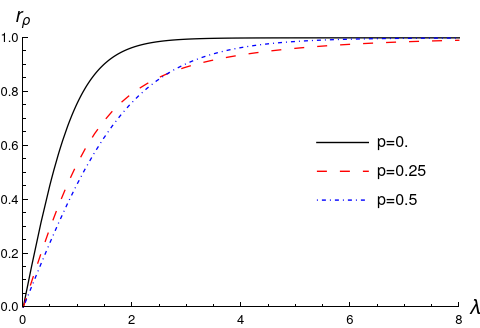
\includegraphics[width=0.8\columnwidth]{figures/r(lambda).png}%
                \caption{$r_{\rho}$ as a function of $\lambda$ for different values of $p$}
            \end{figure}
        \end{column}
    \end{columns}
\end{frame}


\end{document}
